% Figure 5. Surface singularities (printed page 36).
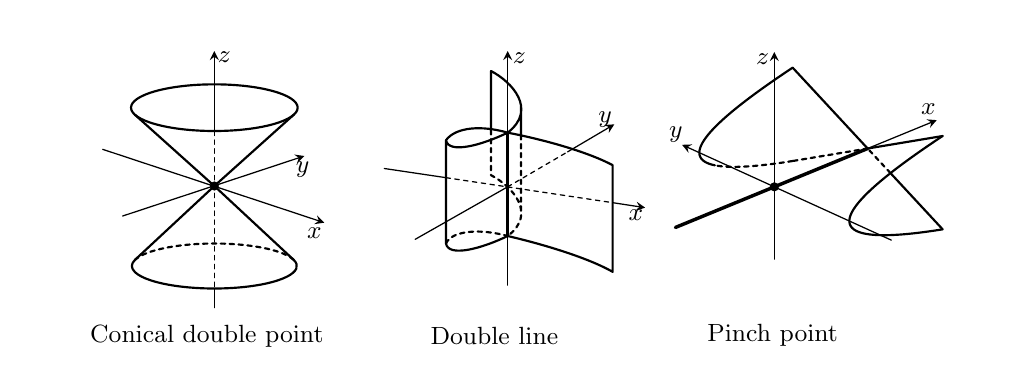
\begin{tikzpicture}[
    x=.3bp, y=-.3bp, line cap=round, line join=round, >=stealth,
    axis/.style={line width=.45bp},
    edge/.style={line width=.78bp},
    singular/.style={line width=1.24bp},
    hidden/.style={dash pattern=on 1.6bp off 1.6bp},
    every node/.style={inner sep=0pt,font=\small}
  ]
  \path[use as bounding box] (-34,-15) rectangle (1129.333,378.333);

  % Conical double point. The far rim of the lower cone is occluded.
  \coordinate (vertex) at (190,175);
  \draw[axis,->] (56,131) -- (322,219);
  \draw[axis,->] (80,211) -- (298,139);
  \draw[axis,->] (190,109) -- (190,13);
  \draw[axis,hidden] (190,109) -- (190,298);
  \draw[axis] (190,298) -- (190,321);
  \draw[edge] (190,81) ellipse[x radius=100, y radius=28];
  \draw[edge]
    (94.54,89.34) -- (vertex) -- (285.46,89.34)
    (95,263.41) -- (vertex) -- (285,263.41);
  \draw[edge,hidden] (285,263.41)
    arc[start angle=-16.33,end angle=-163.67,x radius=99,y radius=27];
  \draw[edge] (285,263.41)
    arc[start angle=-16.33,end angle=196.33,x radius=99,y radius=27];
  \fill (vertex) circle[radius=1.65bp];
  \node at (202,20) {$z$};
  \node at (296,155) {$y$};
  \node at (310,231) {$x$};
  \node at (181,355) {Conical double point};

  % Double line. The two sheets are drawn as vertical extrusions.
  \draw[axis] (394,154) -- (468,165);
  \draw[axis,hidden] (468,165) -- (668,195);
  \draw[axis,->] (668,195) -- (707,201);
  \draw[axis] (431,239) -- (542,176);
  \draw[axis,hidden] (542,176) -- (614,134);
  \draw[axis,->] (614,134) -- (670,101);
  \draw[axis,->] (542,294) -- (542,13);

  \draw[edge,hidden]
    (522,108) -- (522,162)
      .. controls (547,175) and (578,208) .. (542,235)
    (558,114) -- (558,207)
    (468,244) .. controls (475,228) and (510,226) .. (542,235);
  \draw[edge]
    (522,108) -- (522,37)
      .. controls (547,50) and (578,83) .. (542,111)
    (558,79) -- (558,114)
    (542,111) .. controls (589,120) and (640,135) .. (668,150)
      -- (668,278) .. controls (640,262) and (589,246) .. (542,235)
    (542,111) .. controls (511,102) and (480,104) .. (468,120)
      .. controls (471,137) and (511,126) .. (542,111)
    (468,120) -- (468,244)
      .. controls (471,261) and (511,250) .. (542,235);
  \draw[singular] (542,111) -- (542,235);
  \node at (556,21) {$z$};
  \node at (659,95) {$y$};
  \node at (696,210) {$x$};
  \node at (526,355) {Double line};

  % Pinch point. Orthographic projection of (x,y,z)=(s^2,t,st),
  % restricted to |s|,|t|<=1. Smaller x is closer in this view.
  \coordinate (pinch) at (862,176);
  \begin{scope}[
      shift={(pinch)},
      x={(33.6bp,13.8bp)}, y={(-27bp,12.3bp)}, z={(0bp,16.8bp)}
    ]
    \draw[axis,->] (0,-1.56,0) -- (0,1.23,0);
    \draw[axis,->] (0,0,-1.55) -- (0,0,2.89);
    \draw[axis,->] (1,0,0) -- (1.74,0,0);

    % The hidden part of the rim t=1, and the occluded ends at x=1.
    \draw[edge,hidden]
      plot[domain=-1:-.408,samples=24,variable=\s,smooth] ({\s*\s},1,{\s})
      (1,0,0) -- (1,1,-1)
      (1,-.304,-.304) -- (1,0,0);
    \draw[edge]
      plot[domain=-.408:1,samples=32,variable=\s,smooth] ({\s*\s},1,{\s});
    \draw[edge]
      plot[domain=-1:1,samples=42,variable=\s,smooth] ({\s*\s},-1,{-\s});
    \draw[edge]
      (1,-1,1) -- (1,0,0) -- (1,1,1)
      (1,-1,-1) -- (1,-.304,-.304);
    \draw[singular] (-1.06,0,0) -- (1,0,0);
    \fill (0,0,0) circle[radius=1.65bp];
  \end{scope}
  \node at (848,23) {$z$};
  \node at (744,113) {$y$};
  \node at (1047,83) {$x$};
  \node at (860,354) {Pinch point};
\end{tikzpicture}
